\subsection{Overview}
\begin{flushleft}
This section contains a formal model describing the core parts of the system. The model was defined using Alloy, an open-source language and analyzer for software modeling.\\
The purpose of this section is to validate the consistency of the world generated by the union of the previous assumptions and requirements.\smallskip\\

The formal model shows that the system described in the present document is consistent with respect to:
\begin{itemize}
	\item the utilization of the Farmers' Forum.
	\item the send of request from a Farmer to an Agronomist.
	\item the creation and confirmation of an agronomist plan.
\end{itemize}

\end{flushleft}

\subsection{Alloy Model}

\subsubsection{Alloy Code}
\lstinputlisting[language=alloy]{../AlloyCode/DREAMS.als}

\subsubsection{Predicates execution and assertions checks}
\begin{figure}[H]
\centering
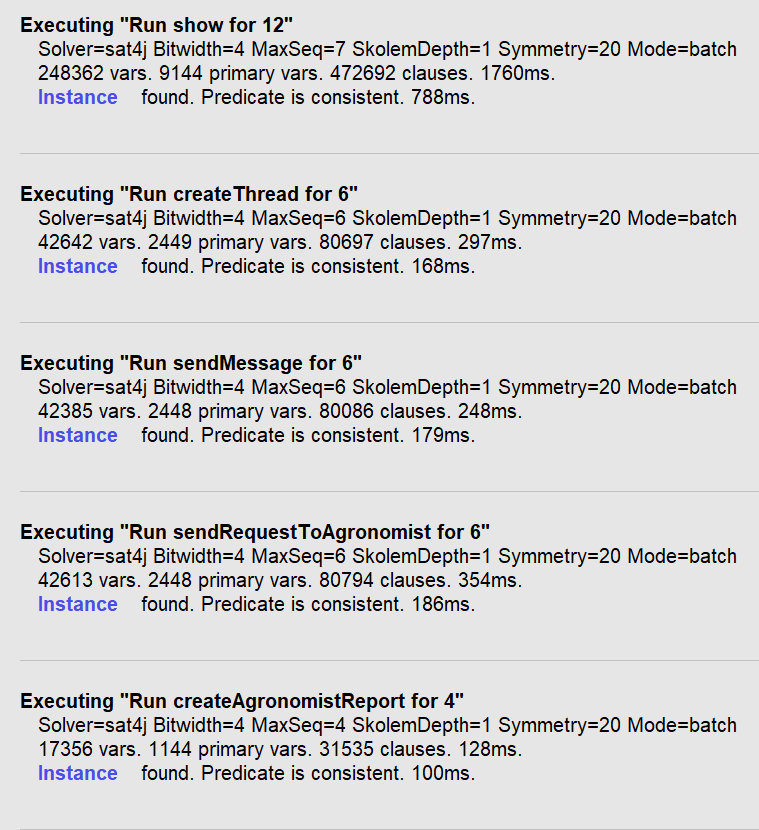
\includegraphics[scale=0.4]{../AlloyCode/executionImages/execution_short1.png}
\end{figure}

\begin{figure}[H]
\centering
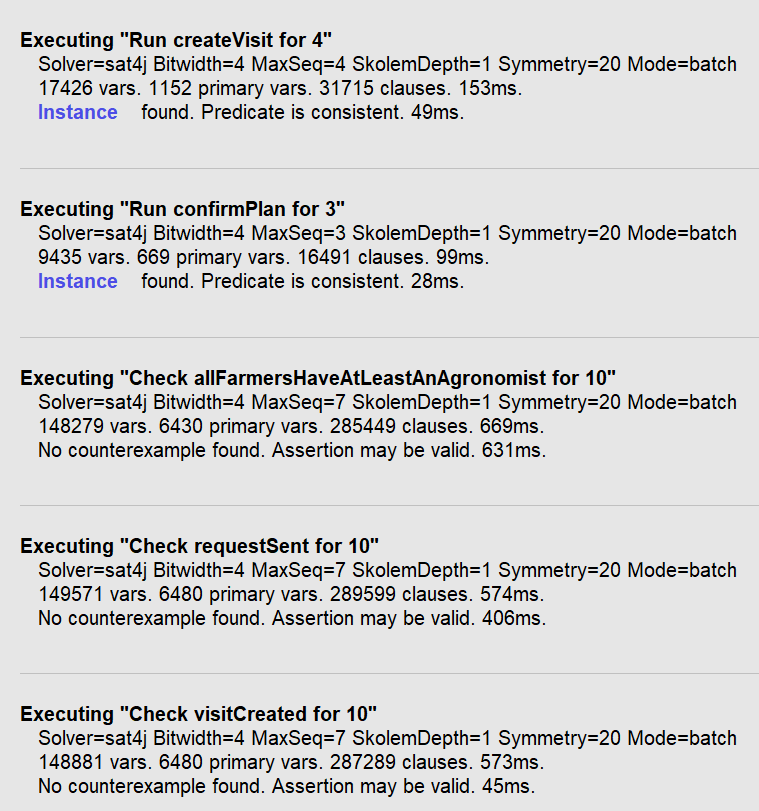
\includegraphics[scale=0.4]{../AlloyCode/executionImages/execution_short2.png}
\caption{\label{fig:alloyExecution}Execution of 7 predicates and check of 3 assertions.}
\end{figure}

\newpage
\subsection{Worlds generated}
To better represent the model described above, we decided to show all the elements only in the first World. With World 2 and following, we show different sections of the model more significant to our purpose.

\subsubsection{World 1}
In World 1 we include one element for each signature. It is possible to see the complexity described by the Alloy and how it is consistent.

\begin{figure}[H]
\centering
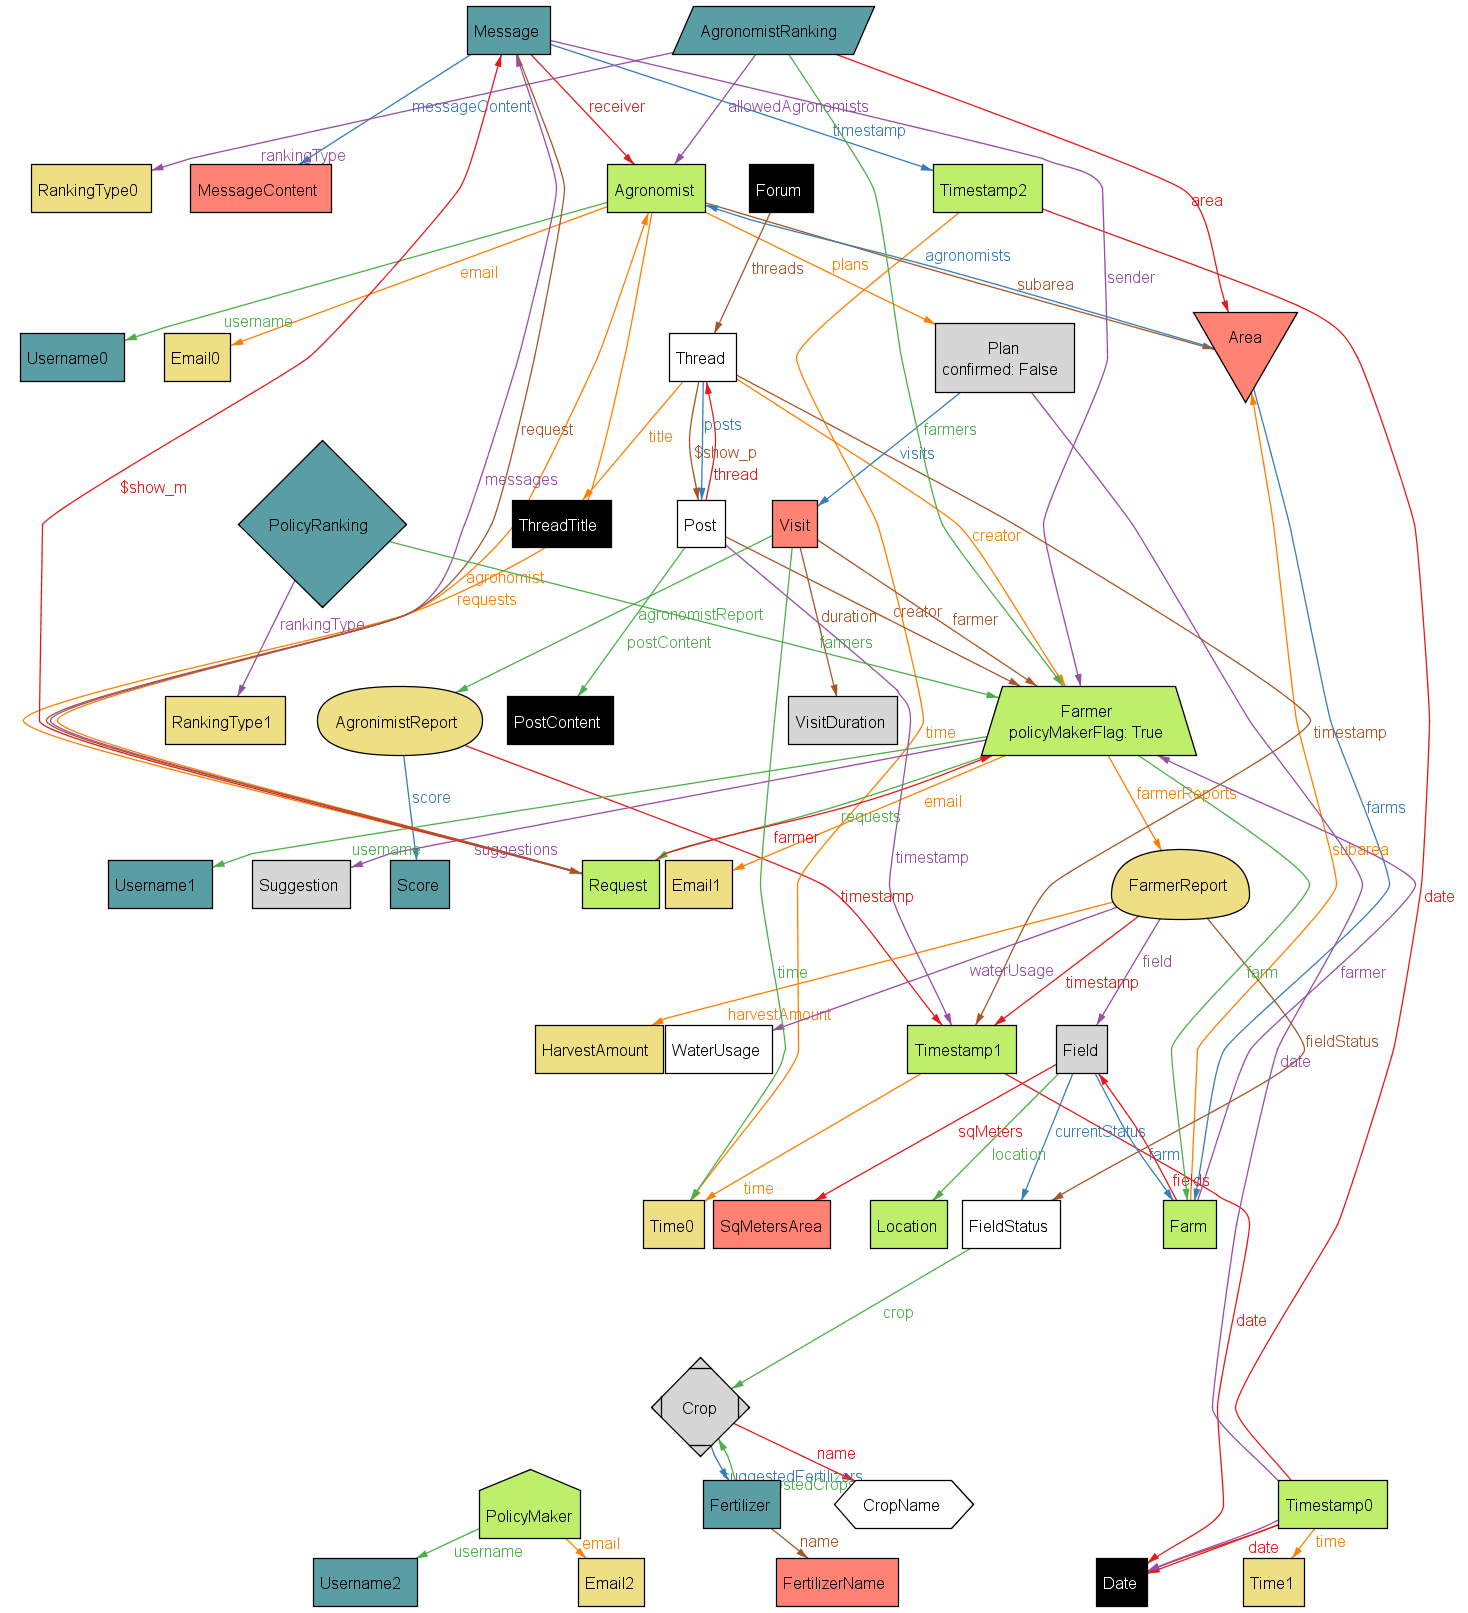
\includegraphics[width=\textwidth]{../AlloyCode/ExportWorldPNG/world1_all.png}
\caption{\label{fig:alloyExecution}World 1 - Complete model}
\end{figure}

\subsubsection{World 2}
In this world we show some farmers sending requests for help to the agronomists and how they can interact with each other exchanging messages.

\begin{figure}[H]
\centering
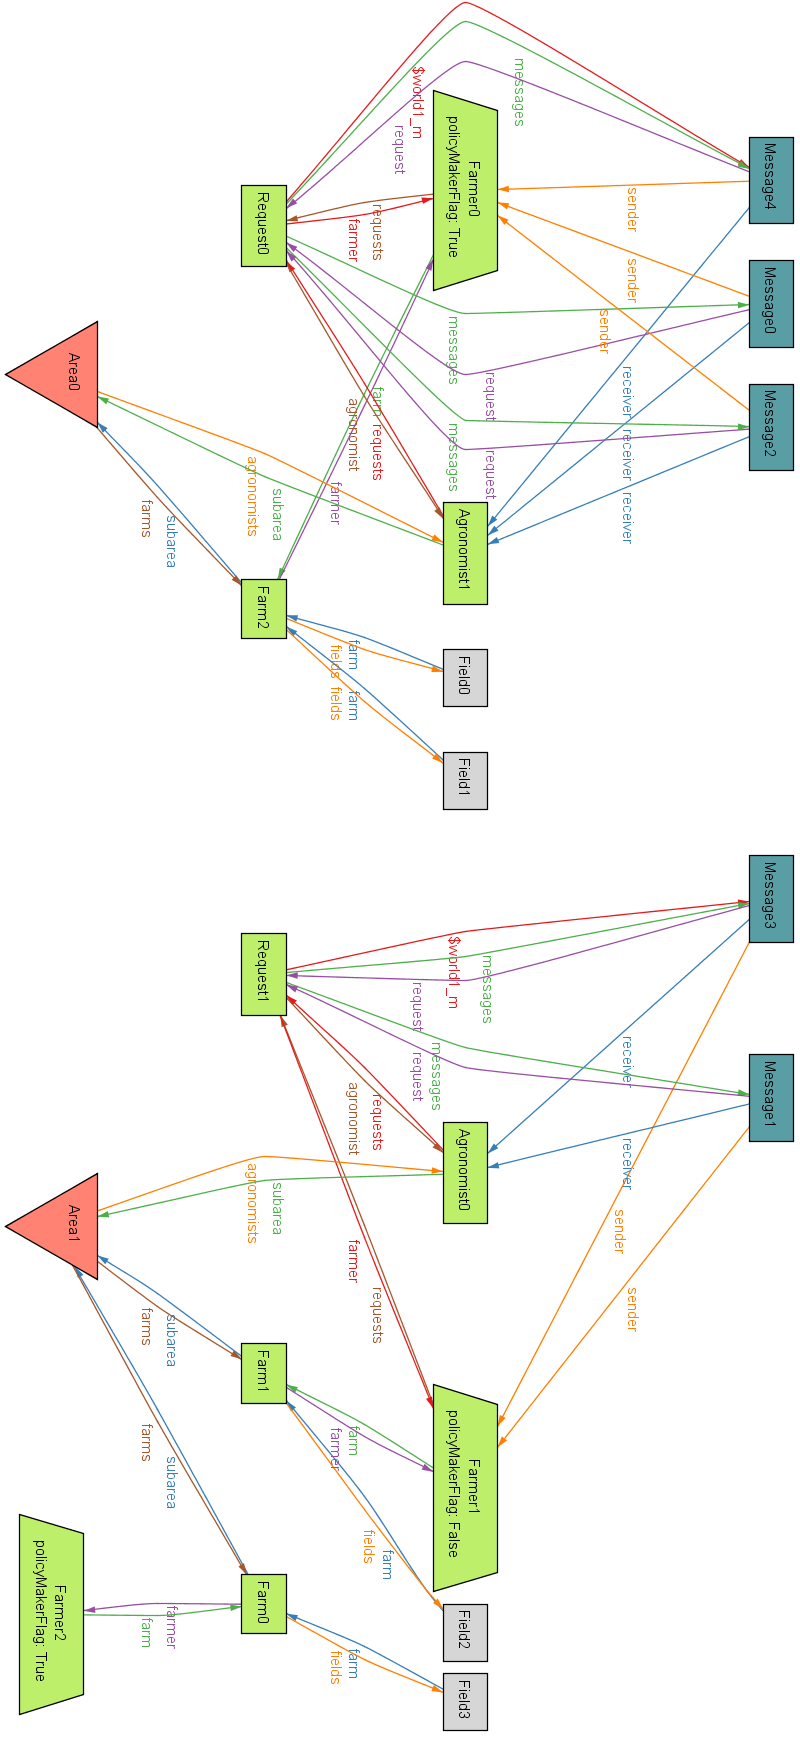
\includegraphics[scale=0.34]{../AlloyCode/ExportWorldPNG/world2_farmer_agro_requests.png}
\caption{\label{fig:alloyExecution}World 2 - Farmer, Agronomist and Request}
\end{figure}

\subsubsection{World 3}
In this world instead, we decided to represent many different elements: first of all the daily plan creation and confirmation for the agronomist.\\
It is possible to see also the reports issued by the agronomist after each visit and both the agronomist and policymaker ranking.
The latter contains the list of all the farmers, instead, the agronomist' one is restricted to only the area in which the agronomist belongs.
\begin{figure}[H]
\centering
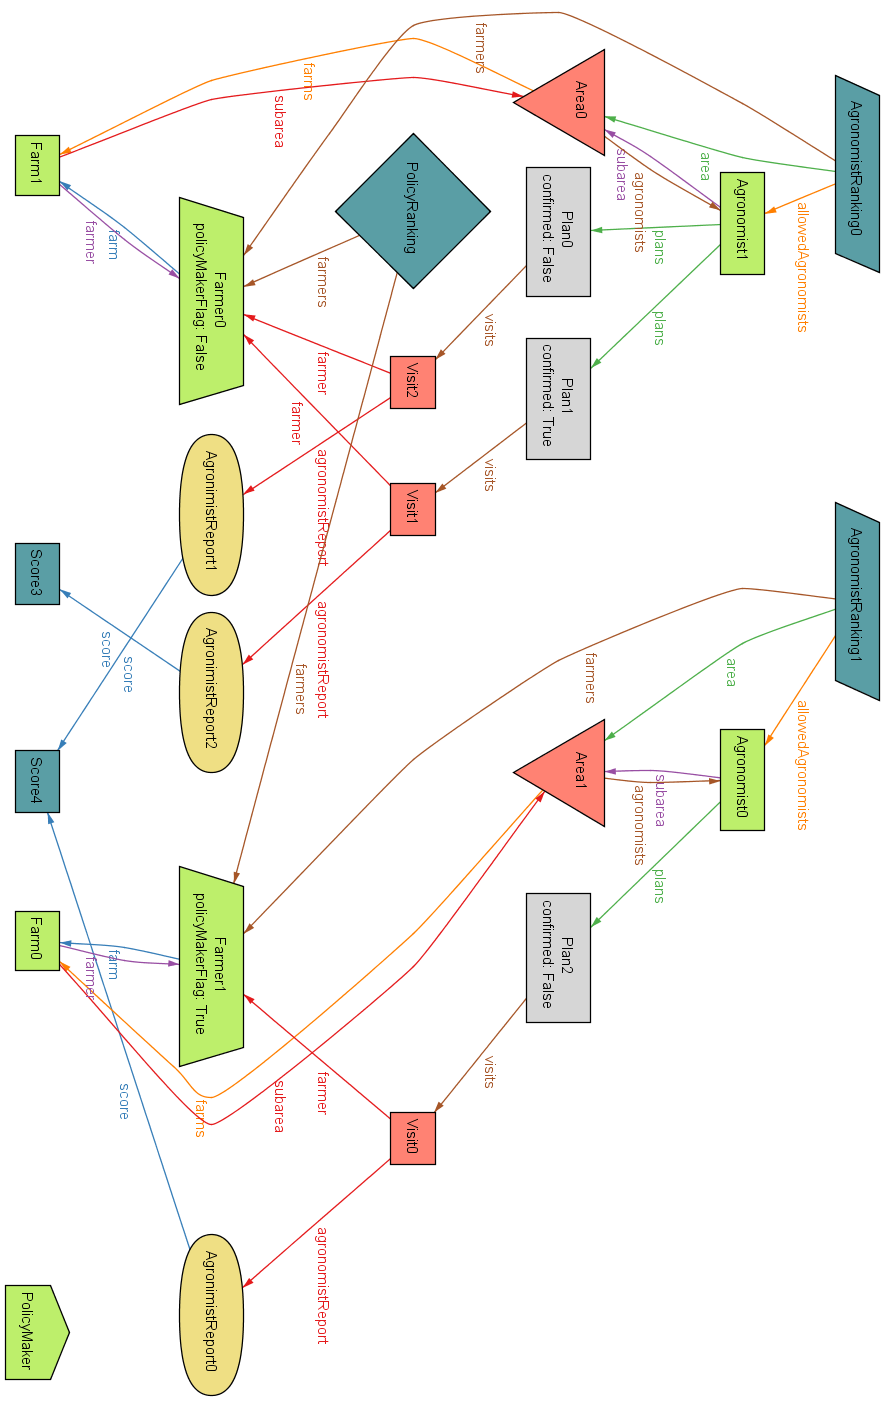
\includegraphics[scale=0.4]{../AlloyCode/ExportWorldPNG/world3_agro_policymaker_reports_rankings.png}
\caption{\label{fig:alloyExecution}World 3 - Agronomist, Policy Maker and Rankings}
\end{figure}

\subsubsection{World 4}
In this last world we wanted to show the functionality of the Farmers Forum with different threads and posts. Each post has its own creator and belongs to only one thread.
\begin{figure}[H]
\centering
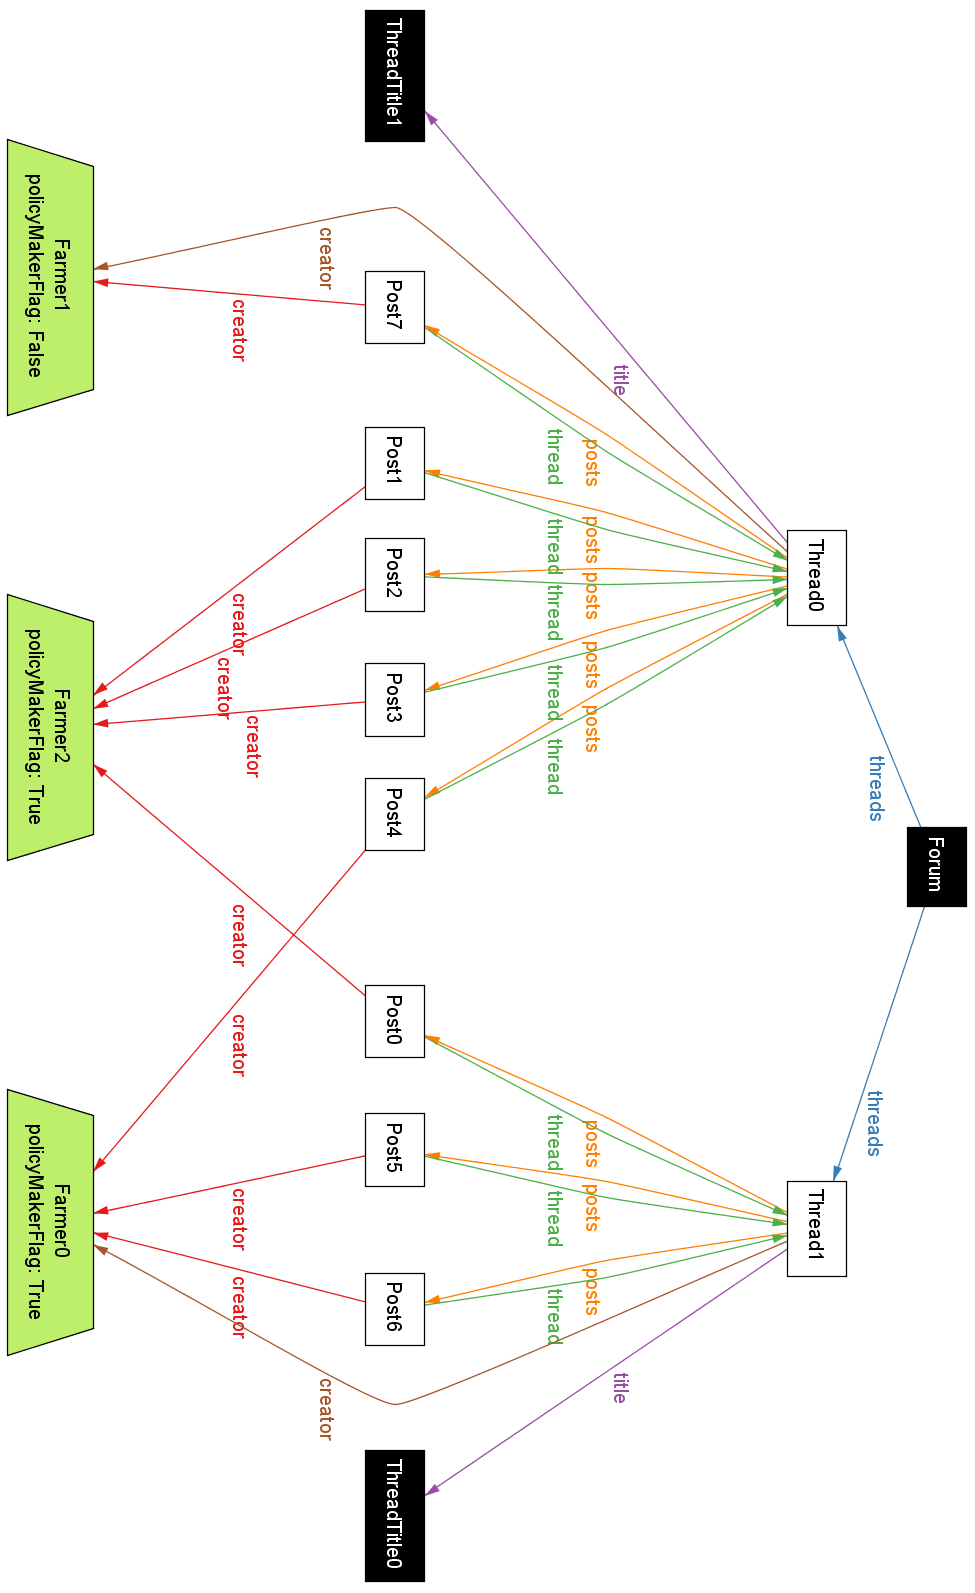
\includegraphics[scale=0.37]{../AlloyCode/ExportWorldPNG/world4_farmer_forum.png}
\caption{\label{fig:alloyExecution}World 4 - Farmer and Forum}
\end{figure}
